% Metódy inžinierskej práce

\documentclass[10pt,twoside,slovak,a4paper]{article}

\usepackage[slovak]{babel}
%\usepackage[T1]{fontenc}
\usepackage[IL2]{fontenc} 
\usepackage[utf8]{inputenc}
\usepackage{graphicx}
\usepackage{url}
\usepackage{hyperref}
\usepackage{cite}


\pagestyle{headings}

\title{Gamifikácia ako nástroj motivácie v športoch

\author{Matej Drienovský\\[2pt]
	{\small Slovenská technická univerzita v Bratislave}\\
	{\small Fakulta informatiky a informačných technológií}\\
	{\small \texttt{xdrienovskym2@stuba.sk}}
	}

\date{\small 19. september 2022}
\thanks{Semestrálny projekt v predmete Metódy inžinierskej práce, ak. rok 2022/23, vedenie: Ing. Igor Stupavský}} 


\begin{document}

\maketitle

\begin{abstract}

Hlavným cieľom tohto článku je vniesť viac svetla do aspektov
gamifikácie. Najmä
v športovom kontexte. Vysvetlenie a oboznámenie, s pojmom gamifikácia. Jej účinok na
ľudskú psychiku. Jej základné využitie v rôznych športových aplikáciách, cez rôzne možnosti
napredovania pomocou levelov, získavania ocenení, spĺňania vopred určených cieľov,
porovnávania svojich výkonov s ďalšími použivateľmi aplikácie. Vplyv gamifikácie na športový
výkon, pomôcka k napredovaniu oproti ostatným. Prvky gamifikácie, a ako nás motivujú. Použitie aplikácií pri konkrétnych športoch, pri tvorbe zápasov
(matchmaking).
\end{abstract}


\section{Úvod}
Veľké množstvo ľudí hľadá aktivitu na vyplnenie voľného času, odreagovanie sa od práce, školy a podobne. Vo väčšine prípadov ich to zavedie k športu. 
Vďaka rozmachu informačnokomunikačných technológií sa mobilné zariadenia a senzory stali pevnou súčasťou každodenného života.
V dnešnej dobe je všetko realizované prostredníctvom aplikácií v smartphonoch. 
Môžme predpokladať, že ľudia používajú aj športové aplikácie \ref{aplikácie}, ktoré ich motivujú k lepším výkonom alebo umožnia lepšie sledovanie pokroku.\ref{gamifikacia v športoch} Aplikácie zbierajú dáta zo senzorov v zariadení a následne ich vedia vyhodnotiť.
Princípy aplikácií, ktoré nám uľachčia tvorbu zápasov pri turnajoch a iných športových podujatiach.\cite{Effect_of_gamification-Framework}


\section{Gamifikácia} \label{gamifikácia}

\begin{figure*}[tbh]
Gamifikácia je aplikácia herných dizajnových prvkov a herných princípov v neherných kontextoch. Môže sa tiež definovať ako súbor aktivít a procesov na riešenie problémov pomocou alebo za použitia charakteristík herných prvkov. Gamifikácia bežne využíva herné dizajnové
prvky pre zlepšenie produktivity organizácie, učenie, crowdsourcing, nábor a hodnotenie zamestnancov, fyzické cvičenie, dopravné priestupky,voličská apatia,a viac. Zbierka výskumov o gamifikácii ukazuje, že väčšina štúdiío gamifikácii zistila, že má pozitívne účinky na jednotlivcov.


\subsection{Motivácia} 

Ako bolo zmienené, princípy gamifikácie motivujú ľudí k častejšiemu používaniu aplikácie a dávajú impulzy k dosiahnutiu cieľov. Tieto princípy tu budú vysvetlené podrobnejšie. 
\label{prvky} Prvky gamifikácie sa delia do troch kategórií :
\begin{itemize}
  \item {Komponenty}
  \item {Mechanické}
  \item {Dynamické}
\end{itemize}
Komponenty sú základné prvky, ktoré sa používajú pre každý iný prvok vysokej úrovne. Hlavné komponenty
\begin{itemize}
  \item {Body}
  \item {Odznaky}
  \item {Rebríčky}
\end{itemize}
\end{figure*}
\begin{figure*}
    
Na základe modelu aplikácie Hook (Liu Li, 2016) \cite{Improving_motivation-Framework} poskytujú športové aplikácie oznámenia v súvislosti s plánovaným tréningom. Niekto dostane upozornenie že priateľ práve absolvoval tréning, zablahoželá mu. Notifikácie sú prítomné, aby používateľ otvoril aplikáciu a vykonal určitú činnosť. Hlavným cieľom každej aplikácie je, aby používateľ sledoval aktivity súvisiace so športom a budoval si kontakty s inými športovcami.
\end{figure*}
\section{Gamifikácia v športoch} \label{gamifikacia v športoch}
\subsection{aplikácie} \label{aplikácie}

Gamifikačné prvky \ref{prvky} v športových aplikáciách sú kľúčovými prvkami na zmenu správania používateľov.
Vo všeobecnosti sú aplikácie založené na spätnej väzbe a odmenách (napr. Strava, Nike+ Run, Runkeeper). 
Existujú však aplikácie, ktoré majú trochu iný prístup. Zombies Run, kde bežec vidí na obrazovke, kde sú zombie, aby vedel, ktorým smerom má bežať, aby ho zombie nechytili. 
Ďalším príkladom je Spotify, aplikácia na streamovanie hudby, ktorá má funkciu výberu hudby v rámci daného žánru, ktorá zodpovedá tempu behu používateľa.
Na základe myšlienky hudby poskytuje aplikácia Rock My Run vybrané skladby, ktoré zodpovedajú tepovej frekvencii a krokom športovca. 
Počas športovej aktivity sú najčastejšie používanými hernými prvkami okamžitá spätná väzba a sledovanie postupu. 
Aplikácie majú vo všeobecnosti zjednodušené používateľské rozhranie, zatiaľ čo športovec sleduje tréning, aby používateľovi poskytli najdôležitejšie údaje a trendy (napr. rýchlosť, vzdialenosť, polohu).
Ak používateľ vytvoril trasu, ktorú má počas tréningu sledovať, zobrazuje sa ukazovateľ pokroku. V službe Strava je možnosť zapnúť funkciu živého segmentu, ktorá športovcovi umožňuje vidieť štatistiky rovnako, ako keby tam boli všetci ostatní pretekári.Takmer ako vo videohre.
Ako už bolo spomenuté, po absolvovaní tréningu sú v týchto aplikáciách najsilnejšie spätné väzby a mechanizmy odmeňovania.
Od skúsenostných bodov, cez Fuel Score Nike až po trofeje a rôzne druhy meraní sa používajú na poskytnutie presnej spätnej väzby o tréningu. Tieto prvky pomáhajú pochopiť a zvýrazniť kľúčové body tréningu, napr. najrýchlejšie kolo, osobný rekord, najdlhší tréning.
Niektoré aplikácie odmeňujú používateľov udeľovaním odznakov, ak splnia určitú výzvu. 
Výzvy môžu fungovať ako spúšťač pre používateľov pridaním časového limitu a cieľa na dokončenie.
 Niekedy sa tieto výzvy týkajú skutočných udalostí, ako je Tour de France alebo Mount Everest, napr. zdolanie výšky Mount Everestu bicyklom alebo behom a získanie odznaku.
Tieto udalosti môžu poskytnúť príbeh tréningu, čím ho robia zaujímavejším a pútavejším pre použivateľa. Športovec sa zžije s príbehom a bude sa snažiť športovať viac a viac.
Zozbierané odmeny, odznaky sa zvyčajne vystavujú na na úvodnej strane konta použivateľa alebo v špecialnej sekcii na to určenej. Vystavené odznaky a trofeje sa vystavujú verejne, takže si ich môžu ostatní použivatelia, priatelia prehliadnuť.\cite{Effect_of_gamification-Framework}

\section{Diagram}
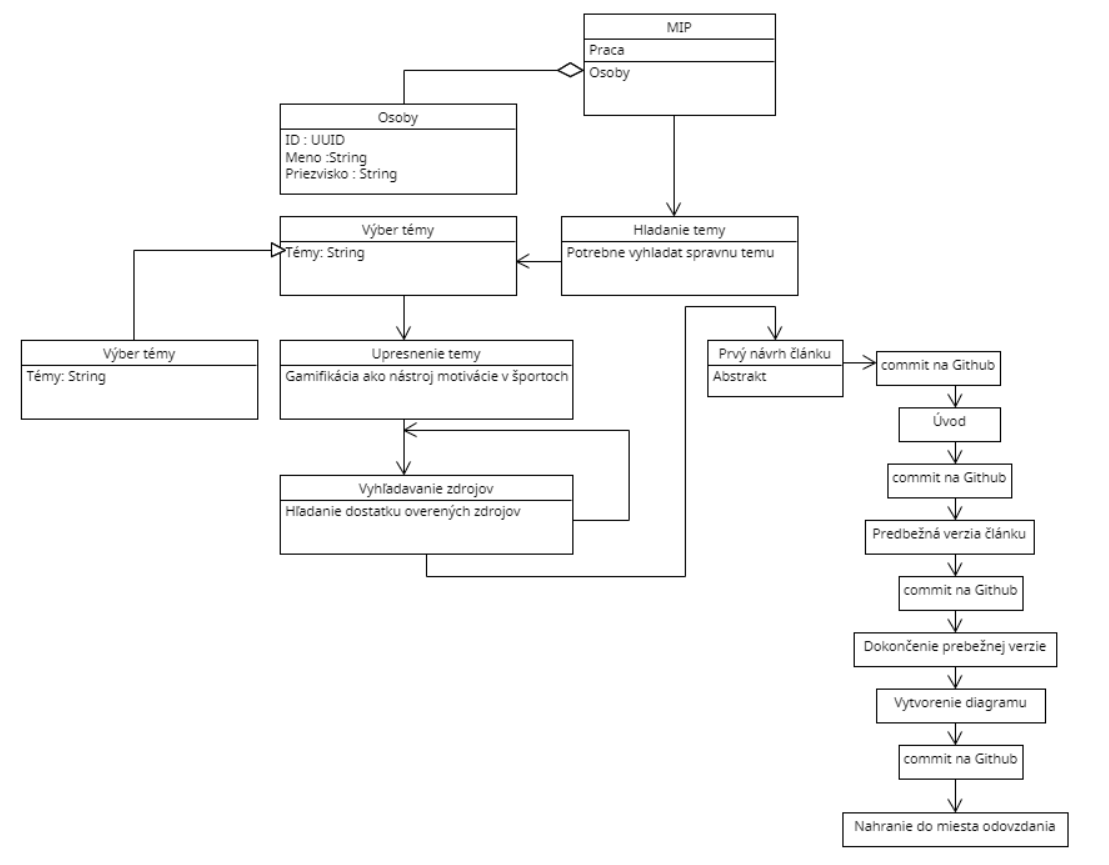
\includegraphics[scale =0.6]{diagram.png}

\bibliography{literatura}
\bibliographystyle{abbrv}
\end{document}
